\section{Potential applications }
\begin{itemize}
\item Art / NFT galleries with instant sales
\end{itemize}

This application allows artists and content creator communities to
display and sell NFT and fungible art to global consumer audiences,
instantly.

\begin{itemize}
\item
  Large scale conference center

  \begin{itemize}
  \item
    Academic conferences
  \item
    Political conference
  \item
    Commercial expo
  \end{itemize}
\end{itemize}

In a hypothetical virtual conference centre a true marketplace of ideas
could be enacted, with participants being paid directly by their
audience based on the proximity to the presentation.

\begin{itemize}
\item
  Group entertainment

  \begin{itemize}
  \item Global social puzzle gaming with prizes
  \item
    Music festivals and gigs - Pay live artists and DJs in real time
    depending on location within the extended landscape of the venue.
    Split to music producer a portion of the value
  \item
    Mixed reality theatre
  \item
    murder mystery
  \item
    Mixed reality live immersive MMORG games
  \item
    Bingo and mass participation gameshows
  \item
    Immersive brand storytelling metaverses
  \item
    Escape rooms
  \end{itemize}
\item
  Debating townhall meetings (with voting etc)
\item
  Mixed reality information metaverse

  \begin{itemize}
  \item
    AR based city tours with collectibles
  \item
    AR based collectibles for trails and heritage (museums, libraries)
    with location specific donations.
  \end{itemize}
\item
  Retail applications

  \begin{itemize}
  \item
    Proxy for physical market
  \item
    AR home delivery market interface within physical marketplaces
  \end{itemize}
\item
  Global course / Education provision
    \begin{itemize}
  \item
    Explore the universe as a group of spaceship or planet characters
  \item
    Explore biology and physics at a microscopic and nanoscopic level
  \end{itemize}
\item
  Micro tasking marketplace
\item
  Code bounty marketplace
\item
  Micro remittance role sharing (business PA / reception etc)
\item
  Careers fair with credential passing
\item
  Auctions in mixed reality
\item
  eSports and live sports
\item
  Gambling, betting markets, and financial leverage markets
\end{itemize}

\subsection{Global cybersec course delivery}
Isolating and building out one example here:
\begin{itemize}
\item Elements for the infrastructure: Economic layer, asset layer, content interface, user management, data storage, microsites loaded in Wolvin and webm, accessibility schema, network security, backups, secure messaging. Deployable framework with high modularity. Some more ossified elements for surity, some less so for malleability and open opportunity. Figure \ref{fig:globalclassroom}.
\item Course delivery in XR, how to we develop a platform, marketplace, framework for open contribution.
\item WebXR, Vircadia, any snap in metaverse middleware that is free and open source (action to compare the two). 
\item Define an interface schema for bolting in any commercial or FOSS metaverse engine.
\item VR marketplace (outside the scope of the VR engine) without a trusted third party.
\item Cryptographically managed learning deliverables (coursework as NFT). 
\item Secure messaging and group messaging using cryptographic keys. Check this stuff with the distributed computing science people in the group (action on John)
\item work toward an exemplar MVP which is then "in the wild"
\item Platform for educators
\item Define scheme, documentation, best practice, interfaces, functional objects, pedagogy, accessibility, multi-language. 
\item Define user management system for educators and client learners.
\item Identify the pain points which current FOSS elements which need development time/money
\item separate the UI/engine from the graphical assets, and the educational / pedagogical components, accessibility, and the value and asset transfer layers.
\item Desktop systems are the primary target (low end system)
\item define schema for accessibility. Colour, subtitles, immersion concerns which can be applied to metaverse rooms through API?
\item Start to define the hybrid presentation model we favour. Avatars? Micro sites? A combination of the two? Balance of guided vs unguided experience. Do we need to test the correct way to do delivery? Is there prior art we can draw on? I feel I should know. Is this part of the research that's being done here?
\item Big work package on schema vs key and user management to enforce rules in spaces. Only participants who have provably paid should have access to learning material, the ability to input into the assessment system, and the tokenised learning outcome `NFT' or proof.
\item Proof that XR system improve learning outcomes. Also that the proposed systems for micro-transactions and user and schema management give additional headroom for teaching.
\end{itemize}
\subsection{Subvocalisation with LLMs}
MIT \href{https://dspace.mit.edu/handle/1721.1/123121}{full thesis} on AlterEgo
\begin{tcolorbox}[enhanced, frame style={fill=lightgray}, interior style={fill=lightgray}]
By transcribing residual neurological signals sent from the brain to speech articulators during internal articulation, the system allows one to communicate without the need to speak or perform any visible movements or gestures. It is capable of transcribing continuous silent speech at a rate of over 100 words per minute. The system therefore provides a natural alternative to normal speech at a rate not far below that of conversational speech. This alternative method of communication enables those who cannot speak, such as people with speech or neurological disorders, as well as those in environments not suited for normal speech, to communicate more easily and quickly. In the same capacity, it can serve as a discreet, digital interface that augments the user with information and services without the use of an external device. I discuss herein the data processing and sequence prediction techniques used, describe the collected datasets, and evaluate various models for achieving such a continuous system, the most promising among them being a deep convolutional neural network (CNN) with connectionist temporal classification (CTC).
\end{tcolorbox}
\subsection{AI 3D objects in metaverse}
Onmiverse from Nvidia apparently have this \href{https://www.nvidia.com/en-us/gpu-cloud/picasso/}{pretty much sewn up}, but they are an expensive \href{https://developer.nvidia.com/blog/rapidly-generate-3d-assets-for-virtual-worlds-with-generative-ai/}{commercial offering}. \par
Notably they now have a \href{https://blogs.nvidia.com/blog/2023/06/27/magiscan-app-augmented-reality-openusd/?}{consumer product}. \par
Industry insiders I have talked to say they thing the Nvidia Omniverse initiative is failing, and this has been my impression too. The results can be seen in Figure \ref{fig:nvidiavoice}.
\begin{figure}[H]
    \centering
    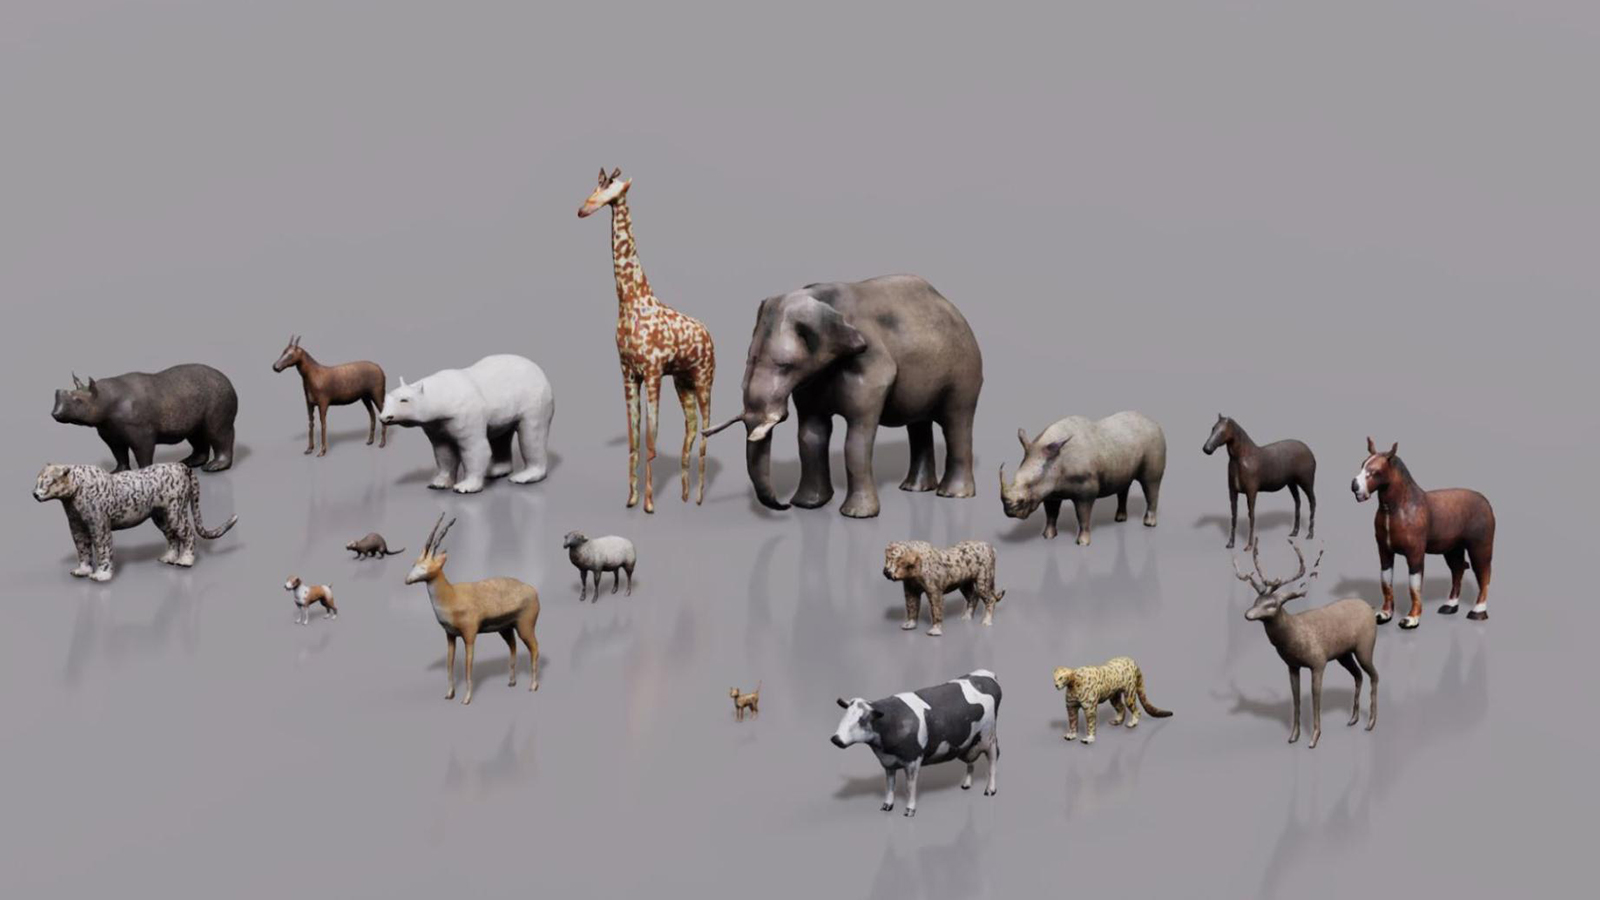
\includegraphics[width=0.95\textwidth]{images/nvidiavoice}
    \caption{Omniverse allows voice created 3D models.}
    \label{fig:nvidiavoice}
\end{figure}
Their voice to facial animation stack Audio2Face is outstanding, but it's unclear how this might challenge Unreal's Metahuman. More promisingly Nvidia have a new video to NeRF to mesh technique called Neuralangelo \cite{li2023neuralangelo} which knocks everything else out of the park. 
\begin{tcolorbox}[enhanced, frame style={fill=lightgray}, interior style={fill=lightgray}]The new AI model by NVIDIA Research for 3D reconstruction using neural networks, turns 2D video clips into detailed 3D structures — generating lifelike virtual replicas of buildings, sculptures and other real-world objects. Like Michelangelo sculpting stunning, life-like visions from blocks of marble, Neuralangelo generates 3D structures with intricate details and textures. Creative professionals can then import these 3D objects into design applications, editing them further for use in art, video game development, robotics and industrial digital twins.
\end{tcolorbox}
This area of 3D generation from various high level inputs is moving \textbf{very} fast and much of the high end stuff is coming as software that can be built on (like NeRF). An open source text to model pipeline for interactively building key assets for pre-viz, or project planning has appeal  \cite{poole2022dreamfusion}.
%All assets can be switched over to Unreal metaverse and become consistent (optimised) digital set which can be visited by stakeholders, funders, VIPs etc. Public can visit later for a fee? Digital assets can be bought from the set. 
There's a lot here but you'd need to be sure that you're not competing directly with Omniverse, by differentiating the product.

\subsection{Digital collectibles for events}
I've been following the NFT and digital objects space since it started, but I have no interest in Ethereum or other NFT technologies because I have been waiting for what I regard as better technology. By luck my preferred option is going live as I write this document, and I am a tester on the programme. I have been talking to those teams since early 2021 and I think I understand it fairly well. There is a first mover advantage here. \href{https://coinmarketcap.com/alexandria/article/bitcoin-is-now-the-second-most-popular-blockchain-for-nfts}{Digital objects on Bitcoin} are the second most popular route after Ethereum now, and might overtake. They split into a bunch of catagories:
\begin{itemize}
\item Ordinals inscriptions, which I have been following since they were posited. I have minted one successfully, but I consider them wasteful and expensive for commercial projects with large audiences.
\item BRC-20 tokens. These are comparatively new, again leveraging the ordinal technique. All this is written up in detail in my book and it's all over the internet. BRC-20 creates ``batches'' of fungible tokens and can be approximated to event tickets, unique but interchangable within their context. They are trivial to make but I am unsure of the business case as they don't \textit{trigger} that unique thing that people seem to like. They're the new meme pump and dump token of choice, with associated negative press in tow.
\item Taproot Assets. This is working on testnet still I think, and is a naked copy of RGB backed by shifty stablecoin types. Might win because of money, worth watching.
\item Pear credits. I think these are failing to get traction but are an honourable mention.
\item Tokens on Liquid sidechain. Fringe, complex, but very heavily invested in and developing quietly makes this one to watch longer term.
\end{itemize}
My use case for these things has always been the cheap creation of a universal provenance for any and all objects and actions in a persistent digital collaborative space. Unlike Ethereum they're basically free, which opens up huge opportunity space. I can unpack this but it really needs to be application led.
\subsubsection{Preferred options: LNP/BP and RGB}
\href{https://giacomozucco.com/layers-before-bitcoin}{LNP/BP} is a non profit standards organisation in Switzerland which contributes to open source development of Bitcoin layer 3 solutions into the Lightning protocol, and Bitcoin protocol (LNP/BP). One of the core product developments within their work is the \href{https://www.rgb.tech/}{`RGB' protocol}, which is somewhat of a meaningless name, evolved from ``coloured coins'' which were an early tokenised asset system on the Bitcoin network. RGB represents red, green, and blue. The proposal is built upon research by \href{https://petertodd.org/2016/commitments-and-single-use-seals}{Todd} and \href{https://giacomozucco.com/#intro}{Zucco}. RGB is regarded as arcane Bitcoin technology, even within the already rarefied Bitcoin developer communities. Zucco provides the \href{https://bitcoinmagazine.com/culture/video-interview-giacomo-zucco-rgb-tokens-built-bitcoin}{following explanation}: \par
\textit{``When I want to send you a bitcoin, I will sign the transaction, I will give the transaction only to you, you will be the only one verifying, and then we’ll take a commitment to this transaction and that I will give only the commitment to miners. Miners will basically build a blockchain of commitments, but without the actual validation part. That will be only left to you. And when you want to send the assets to somebody else, you will pass your signature, plus my signature, plus the previous signature, and so on.''}\par
This is non-intuitive explanation of Todds `single-use-seals', applied to Bitcoin, with the purpose of underpinning arbitrary asset transfer secured by the Bitcoin network. In this model the transacting parties are the exclusive holders of the information about what the object they are transferring actually represents. This primitive can (and has) been expanded by the LNP/BP group into a concept called `client side validation'. 
It's appropriate to explain this concept several times from different perspectives, because this is potentially a profoundly useful technology for metaverse applications.\par
\begin{itemize}
\item A promise is made to spend a multi output transaction in the future. This establishes the RGB relationships between the parties.
\item One of the pubkeys to be spent to is known by both parties.
\item The second output is unknown and is a combination of the hash of the state, and schema, from the operation which has been performed.
\item When the UTXO is spent the second spends pubkey can be processed against the shared data blob to validate the shared state in a two party consensus  (sort this out, it's nonsense).
\item This is now tethered to the main chain. Some tokens from the issuance have gone to the recipiant, and the remainder have gone back to the issuer. More tokens can be issued in the same way from this pool. 
\item A token schema in the blob will show the agreed issuance and the history back to the genesis for the token holder. 
\item The data blob contains the schema which is the key to RGB functions and the bulk of the work and innovation. 
\item Each issuance must be verified on chain by the receiving party. 
\end{itemize} 
This leverages the single-use-seal concept to add in smart contracts, and more advanced concepts to Bitcoin. Crucially, this is not conceptually the same as the highly expressive `layer one' chains which offer this functionality within their chain logic. In those systems there is a globally available shared consensus of `state'. In the LNP/BP technologies the state data is owned, controlled, and stored by the transacting parties. Bitcoin provides the crytographic external proof of a state change in the event of a proof being required. This is an elegant solution in that it takes up virtually no space on the blockchain, is private by design, and is extensible to layer 2 protocols like Lightning.\par
This expanding ecosystem of client side verified proposals is as follows:
\begin{itemize}
\item RGB smart contracts
\item RGB assets are fungible tokens on Bitcoin L1 and L2, and non fungible Bitcoin L1 (and somewhat on L2).
\item Bifrost is an \href{https://github.com/LNP-BP/presentations/blob/master/Presentation slides/Bifrost.pdf}{extension} to the Lightning protocol, with it's own Rust based node implementation, and backwards compatibility with other nodes in the network. This means it can transparently participate in normal Lightning routing behaviour with other peers. Crucially however it can also negotiate passing the additional data for token transfer between two or more contiguous Bifrost enabled parties. This can be considered an additional network liquidity problem on top of Lightning, and is the essence of the ``Layer 3'' moniker associated with LNP/BP. It will require a great number of such nodes to successfully launch token transfer on Lightning. As a byproduct of it's more `protocol' minded design decisions Bifrost can also act as a generic peer-to-peer data network, enabling features like Storm file storage and Prometheus.
\item \href{https://www.aluvm.org/}{AluVM} is a RISC based virtual machine (programmable strictly in assembly) which can execute Turing complete complex logic, but only outputs a boolean result which is compliant with the rest of the client side validation system. In this way a true or false can be returned into Bitcoin based logic, but be arbitrarily complex within the execution by the contract parties.
\item Contractum is the proposed smart contract language which will compile the RGB20 contracts within AluVM (or other client side VMs) to provide accessible layer 3 smart contracts on Bitcoin. It is a very early proposal at this stage.
\item  Internet2: ``Tor/noise-protocol Internet apps based on Lightning secure messaging
\item Storm is a lightly specified escrow-based bitcoin data storage layer compliant with Lightning through Bifrost.
\item Prometheus is a lightly specified multiparty high-load computing framework.
\end{itemize}
Really, any compute problem can be considered applicable to client side validation. In simplest terms a conventional computational problem is solved, and the cryptographically verifiable proof of this action, is made available to the stakeholders, on the Bitcoin ledger.\par 
Less prosaically, at this stage of the project the more imminent proposed affordances of LNP/BP are described in `schema' \href{https://github.com/LNP-BP/LNPBPs}{on the project github}. The most interesting to the technically minded layperson are:
\begin{itemize}
\item \href{https://github.com/LNP-BP/LNPBPs/blob/master/lnpbp-0020.md}{RGB20} fungible assets. This could be stablecoins like dollar or pounds representation. Bitfinex exchange \href{https://github.com/RGB-Tools/rgb-lightning-sample}{have code} which already works with RGB to transmit Tether stablecoins on testnet. This is a huge application area for Bitcoin, and similar to Omni, which will also be covered next.
\item \href{https://github.com/LNP-BP/LNPBPs/blob/master/lnpbp-0021.md}{RGB21} for nonfungible tokens and ownership rights. In principle BiFrost allows these to be transferred over a the Lightning network, significantly lowering the barrier to entry for this whole technology. DIBA \href{https://diba.io/}{have this technology working} on testnet.
\item \href{https://github.com/LNP-BP/LNPBPs/issues/29}{RGB22} may provide a route to identity proofs. This is covered in detail later.
\end{itemize}
Federico Tenga is CEO of `Chainside' and an educator and consultant in the space. He has written an up-to-date \href{https://medium.com/@FedericoTenga/understanding-rgb-protocol-7dc7819d3059}{``primer''}, which is still extremely complex for the uninitiated, but does capture how the RGB token transfer system works. That medium article also touches on Taro, which is next.
\subsubsection{DIBA and Unique Digital Assets}
\textit{DIBA} is a pioneering digital asset marketplace, powered by the \href{https://www.rgb.tech/}{RGB Smart Contract Protocol}. It permits the creation and direct transaction of Unique Digital Assets (UDAs), akin to Non-Fungible Tokens (NFTs), on Bitcoin without the necessity of other tokens. UDAs are special digital assets linked to a Bitcoin UTXO (unspent transaction output). These assets embody distinctive attributes like ownership, transferability, and divisibility, and remain under the full control and ownership of their creators.\par
Through DIBA, users can explore, purchase, and sell a vast array of UDAs, taking advantage of the robustness and permanence of the Bitcoin blockchain. DIBA's innovation extends to the integration of a Lightning layer 2 solution, aiming to facilitate faster and more affordable transactions.\par
Assets minted via DIBA are bound to Bitcoin's base layer with an on-chain UTXO. They are subsequently stored on the Arweave permaweb alongside a cryptographic hash, which, combined with a digital signature, can validate their authenticity. The RGB Smart Contract Protocol executes UDA transactions via BitMask, a wallet engineered by the DIBA Team.
\subsubsection{BitMask}
\textit{BitMask} is a browser extension wallet birthed by DIBA, intended for decentralized applications on Bitcoin. It grants access to Bitcoin Finance, UDAs, and more, utilizing the RGB protocol. It delivers comprehensive financial autonomy with its taproot-enabled Bitcoin and Lightning Network wallet, establishing it as a gateway to DeepWeb3 on Bitcoin. More details can be found on Bitmask.app.\par
\subsubsection{DIBA's Launch and Marketplace Timelines}
DIBA has initiated an Open Marketplace for Beta testing as of April 2022, available on Bitcoin testnet. The full launch on Bitcoin mainnet is expected to occur in the second or third quarter of 2022. Submissions for the DIBA Curated Marketplace are currently open, allowing interested individuals to apply as an Artist or a Curator.\par
These developments represent a substantial expansion of the capabilities within the Bitcoin network and further attest to the potential of the LNP/BP's work. Notably, DIBA \href{https://diba.io/}{has this technology working} on testnet. The extensive application areas for Bitcoin, such as the transmission of Tether stablecoins on testnet by Bitfinex exchange \href{https://github.com/RGB-Tools/rgb-lightning-sample}{via RGB}, emphasize the potential impact of these advancements.
\subsection{Product Design}
\subsubsection{User Journey}
\begin{itemize}
    \item \textbf{Discovery \& Onboarding}: User downloads and opens the app on their phone or accesses the web application on their computer.
    \item \textbf{Interaction with LLM}: User starts conversing with the open-source AI large language model (LLM).
    \item \textbf{Storyboard Creation}: User co-creates the story arc with the LLM. 
    \item \textbf{Feedback \& Iteration}: User can provide feedback on the story subdivisions and the balance between visual narrative, explanatory text, and dialogue. 
    \item \textbf{Art Style Selection}: User selects an artistic style for the storyboard and provides additional contextual information.
    \item \textbf{Preliminary Image Generation}: The image AI server generates five visual styles based on the chosen art style and additional context.
    \item \textbf{User Interaction with Panels}: The app generates ten blank panels with a small contextual synopsis each.
    \item \textbf{Initial Image Rendering}: The Image AI uses the user-provided data to render ten panels into a single 1024x1024 image.
    \item \textbf{Final Image Rendering \& Text Placement}: The AI subdivides and upscales the chosen image into ten high-quality panels.
    \item \textbf{Final Review \& Confirmation}: After the user has arranged the text to their liking, the AI performs a final rendering pass to create a multi-page comic book-style PDF. 
    \item \textbf{Purchase/Download}: The user has the option to purchase the PDF as a DIBA-based NFT (UDA), or simply save it to their phone or computer.
\end{itemize}

\subsubsection{Technical Overview}
\begin{itemize}
    \item \textbf{Frontend}: A web and `progressive web app' mobile interface with a clean, intuitive style for user interaction.
    \item \textbf{Backend}: The application leverages an open-source LLM trained through Lora and aligned with new \href{https://arxiv.org/abs/2306.17806}{CFG techniques}, for the narrative portion of the comic. This will run on a Lamda cloud compute system, initially an A100 and as the user base scales an H100. It also uses a highly capable Nvidia H100 based server system with open-source generative art capabilities (\href{https://github.com/comfyanonymous/ComfyUI/blob/master/script_examples/basic_api_example.py}{ComfyUI API} for image rendering. The rental cost per year of these systems is around \$30k, without administration costs.
\end{itemize}

\subsubsection{User Stories}
\begin{itemize}
    \item As a user, I want to interact with an AI to create a storyboard so that I can craft a narrative that matches my vision.
    \item As a user, I want to provide feedback on the AI-generated subdivisions of my story to ensure they align with my creative goals.
    \item As a user, I want to choose an art style for my storyboard to suit my aesthetic preferences.
    \item As a user, I want to draw and add descriptive text to my panels to give more context to the AI.
    \item As a user, I want to choose my favourite among multiple AI-generated renderings to have a say in the final visual output.
    \item As a user, I want to arrange text assets on my storyboard to ensure the narrative flow and visual balance is to my liking.
    \item As a user, I want the option to buy my storyboard as a NFT or save it to my device for maximum flexibility in how I use and share my creation.
\end{itemize}
%\section{Conclusion}
%This will follow as the second week develops.
%\lipsum[10]
%This approach to decision making, which is based on a decision matrix, provides a structured, visual way to compare different ideas based on multiple criteria. It allows us to continuously refine and improve our ideas based on feedback from the team, and it provides a clear, visual representation of the strengths and weaknesses of each idea.
